\chapter{Design and Implementation}
\label{chap:cran_for_lora}

In this section we will be elaborating and reasoning the design decisions taken in order to materialize the idea of IoT based surveillance with the blockchain technology. In the first part we will be discussing in detail the different approaches, technologies and communication protocols considered throughout the design decisions. We will also see how the IoT surveillance system with access control drives the design decisions. 

In the second part the design decisions taken will be put into action by implementing the architecture. A number of APIs and data structures are used to materialize the idea however still the Esp Eye device comes with limitations such as the max array size and due to which a dynamic memory allocation is needed.  





\section{Hardware Components}

Before digging deeper in this section we would like to describe the hardware architecture and its components involved in the project.
The video surveillance for face detection and recognition is handled by ESP EYE where the testing environment is based on an AMD Processor machine which can be Windows/Linux/Mac.
In Figure~\ref{fig:hardarchitecture} on the left hand side we have multiple Esp devices which communicate with the IoT gateway within the same network with Wi-Fi based on IEEE 802.11 standards for communication protocols. 

\begin{figure}[!htb]
    \centering
    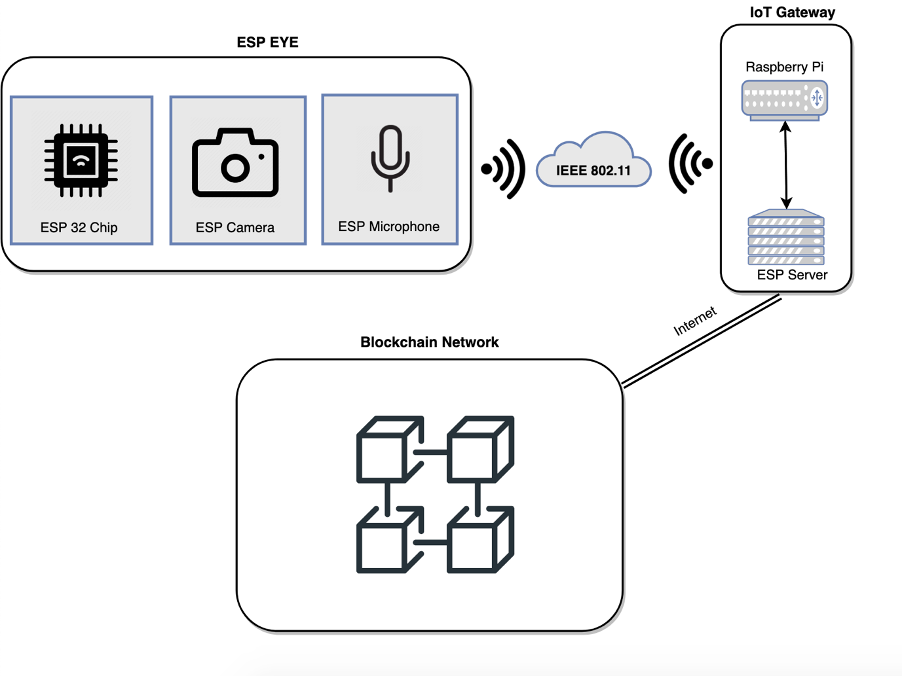
\includegraphics[width=1\textwidth]{figures/surveillance1.png}
    \caption{Hardware Architecture}
    \label{fig:hardarchitecture}
\end{figure}


The IoT Gateway serves as the middle man which waits for images coming from Esp Eye to be inserted into the blockchain. As the main experimental devices in our project we have Esp Eye and the raspberry Pi. But due to experimental purposes we had to run the blockchain locally and that lead us to change the infrastructure and instead of the raspberry pi which is an ARM based processor machine we had to go for AMD based processor machine. This is due to the Hyperledger Fabric which runs in form of containers and its binaries are only available for an AMD processor. However the architecture in the Figure~\ref{fig:hardarchitecture} still holds true. 


\subsection{Esp Eye for Face Detection}

ESP EYE which can be seen in Figure~\ref{fig:espeye} is an AI development board which is based on ESP32 chip. The device was first for sale in 2020 by the semiconductor company Espressif. There are many other devices which are based on the ESP32 family of chips. ESP32 is combine with extra components such as programming interfaces, different sensors which are used for the evaluation of the chip. 
At the core of the board is the dual core Tensilica LX6 processor with 8 MB PSRAM and a 4MB flash. 

The Esp Eye integrates an embedded microphone and a camera with 2-Megapixels. The camera is an OV2640 sensor with a maximum image size of 1600×1200 pixels. The board supports  2.4 GHz Wi-Fi technology to connect to internet through a wide area network. A Micro USB port provides the power supply and also debugging in order to use the AI APIs. It comes with an UART Chip which enables asynchronous serial communication with which the program is uploaded bits by bits. 
\begin{figure}[!htb]
    \centering
    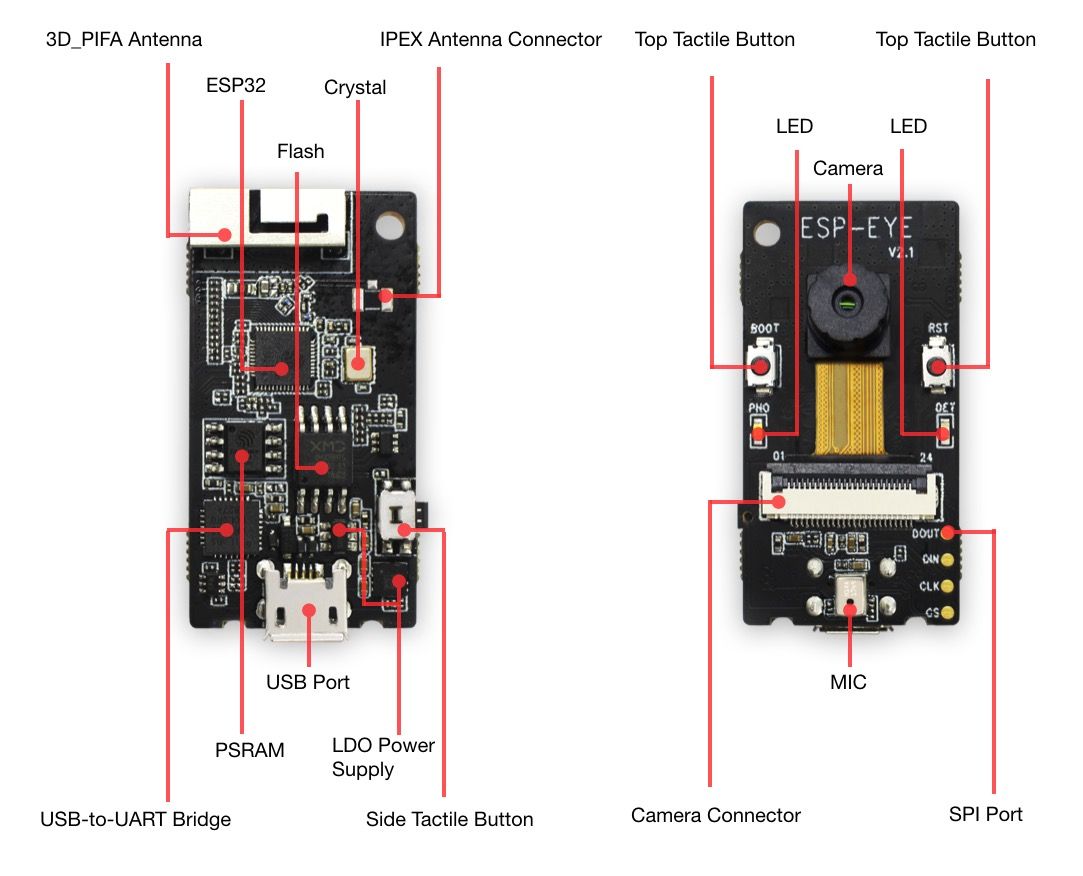
\includegraphics[width=1\textwidth]{figures/espeye.png}
    \caption{Esp Eye}
    \label{fig:espeye}
\end{figure}


Esp Eye also supports additional security features: flash encryption feature and secure boot. The flash encryption is intended to secure the content of the flash memory. In Esp Eye flash encryption is done using AES-256 and the key is stored in the eFuse. eFuses keep the values intact and can not be changed by a software. Since the data in flash is encrypted upon reboot the physical readout will be impossible. 
On the other hand secure boot can protect the device from uploading unsigned code. The algorithm is a typical digital signature method with RSA, the public is stored in the device itself whereas the private is kept secret and used upon each code upload. 

What makes the Esp Eye stand out of the crowd is its performance and the platform for face detection and recognition known as Esp-Who. Esp-who comes with algorithms for face detection and recognition which makes it possible to run both in Esp Eye.

\subsection{Raspberry PI}

Raspberry Pi has been the development environment from the beginning of the project. It is very lightweight, supports many compilers and makes it ideal for experimental purposes. Throughout this project we have been using Raspberry Pi 4 Model B, with 8GB of RAM with  integrated 802.11 wireless LAN. It worth mentioning that the Raspberry Pi is backed by an ARM processor. 
The esp32 family of devices are natively compiled and developed by the esp idf development platform.  Similarly also the Esp-Who libraries for face detection and recognition were available in esp idf development platform.
However after many tries to setup Hyperledger Fabric in Rasperry Pi we realized that Hyperledger Fabric binaries were not possible to run in ARM processor. Therefore after that a computer with AMD processor was used. 






\section{Design}

 


\subsection{Surveillance System Architecture}

Figure~\ref{fig:surveillance2} shows a high level overview with the sotware components. It is important to mention that the design is compatible without any technological restrictions. At the beginning there were two approaches in mind: deployment of face detection and recognition on the cloud or deployment in the Esp Eye device itself. In the first approach AI is deployed on the cloud which means the camera consequently captures images and send them on the cloud for face recognition. This approach is costly, based on the previous studies in average the time required to detect a person is between 2 to 5 seconds. In addition it requires substantial amount of bandwidth which would be wasted if no one is present.

In the second approach which we decided to implement the face detection and recognition run on the IoT device itself. This approach has a lot more benefits, first of all the images are captured by a very small devices powered by AA batteries. Compare to the previous approach they needed a machine on the cloud and a separate camera, whereas in this case both are converged into one single low powered device. When images are captured they are immediately detected and recognized. Which means that it can also be optimized to delete images when a face is not detected. 



\begin{figure}[!htb]
    \centering
    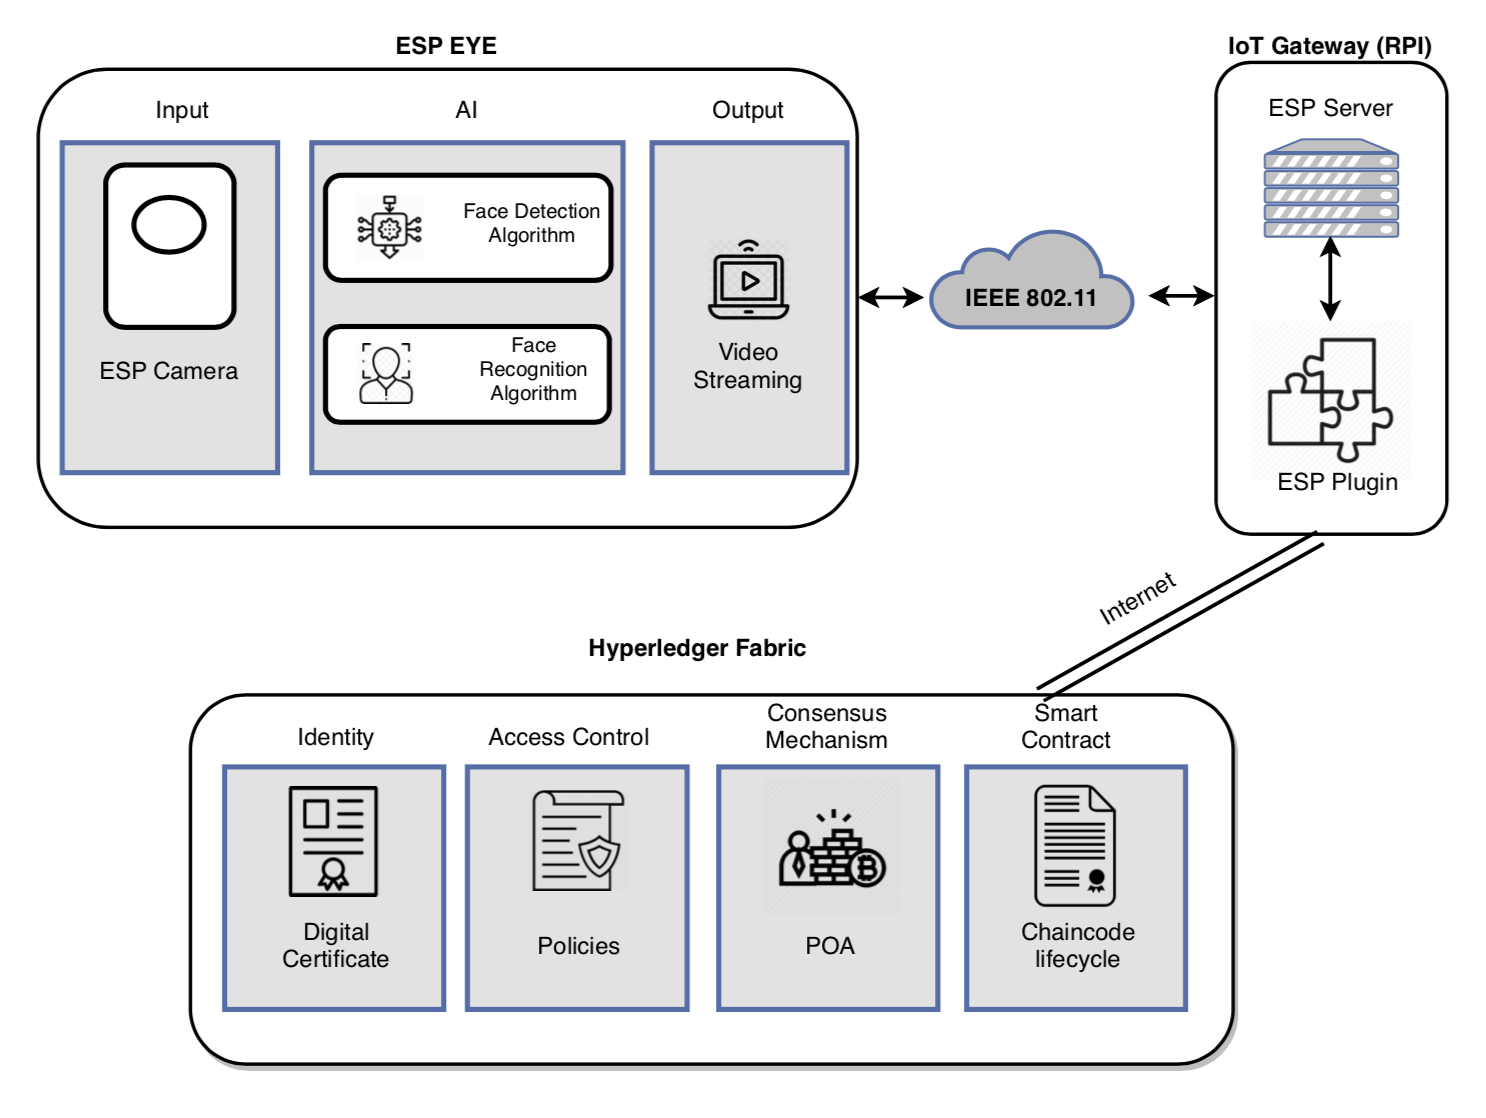
\includegraphics[width=1\textwidth]{figures/esp2.png}
    \caption{Software Architecture}
    \label{fig:surveillance2}
\end{figure}


On the right hand side of the Figure~\ref{fig:surveillance2} is the IoT Gateway which serves as a hub to do the rest of the job. The communication between the Esp Eye and the IoT gateway is achieved with a wireless communication compliant to IEEE 802.11 LAN protocols. It follows the client-server architecture, the Esp Eye is the client and the IoT Gateway as a server. Since we want to store the detected images in the blockchain having the Esp Eye as a client fulfills the requirements. The server will be waiting for requests coming from the Esp Eye. The other way around would not work, since the only way to send data from the server is when the client has sent a request. The first condition for the image to be stored in blockchain is that the face has to be detected in that image. On the other hand ESP Plugin with the help of the SDK from Hyperledger Fabric will start the process of submitting the transaction to the ledger. Hyperledger Fabric enables the storage of the detected images coming from the Esp Eye.   

\subsection{Communication Protocols under consideration}
When it comes to decision which communication protocol to use in IoT device, it is important to go for a lightweight protocol and among our choices is HTTP and MQTT both of them supported by Esp Eye with the help of IPEX antenna which enables the Wi-Fi connectivity. MQTT is an extreme lightweight protocol which follows the publish/subscribe model for communication. Whenever a client pushes a message on a subscribed topic then the message will be forwarded to all the clients participating on that topic. Due to the use case where the esp eye devices do not have to communicate in between the MQTT leaves behind. 
Instead HTTP protocol is employed where Esp Eye and the IoT Gateway communicate in the client server architecture respectively. For the inter-machine communication the REST architectural style will be used because anyways we do not want to bind the communication since we do not know when the face will be detected. Besides REST is considered to be more lightweight compare to its counterparts. For the data-interchange format the JSON format is employed which is very lightweight and performs much better since its syntax follows the javascript language so it makes it faster to read since the ESP server is also written in javascript.  
\subsection{Face detection and recognition algorithms in Esp Eye}
Although very small in size the Esp Eye still stands out of the crowd because of its features and communication standards. With 8 MB of PSRAM and 4 MB and Wi-Fi transmission of flash it gives room for deploying ESP-WHO a platform and a library for face detection and recognition. ESP-WHO is a framework and library which provides the face detection and recognition algorithms. It is developed using the ESP IDF an SDK with software development tools which includes compiler, debugger and some plugins to integrate with additional IDEs.  ESP IDF contains the essential software libraries for the face detection with MTCNN and MobileNets model and face recognition libraries implemented with MobileFaceNet model. In order to elaborate how face detection and recognition works we have Chapter 3 which explicitly explains the used models. 

Although we could have used ESP IDF development environment but rather we chose to develop it in Arduino IDE. Arduino IDE provides a lot of libraries including the libraries for ESP32 boards. 



\subsection{Hyperledger Fabric a tamper-resistant database}

  The main criteria were that the blockchain ought to be private and permissioned since the images should not be public and only available from within the organisation that applies our use case. Ethereum and Hyperledger Fabric was another potential candidate to be deployed.Among the two we decided for Hyperledger Fabric because from the beginning it is meant to be private permissioned blockchain. Although Ethereum can be adapted to serve our needs but yet it comes with a consensus mechanism which is energy demanding and not flexible. Hyperledger Fabric provides a modular architecture and enables more flexibility and is tailored to the needs of our use case. For a better undestanding of the architecture of Fabric you can refer to Chapter 4.  Hyperledger Fabric in our case stands out of the crows due to its features: 

\begin{itemize}
    \item High transaction throughput
    \item Low latency for transaction confirmation
    \item Confidentiality of transactions with the help of channels
    \item Highly modular architecture
    \item Identities supplied with digital certificate 
\end{itemize}

With its modular architecture it allows to be tailored to the needs and the use case. It has been designed to be highly configurable and offers modularity for the following components: 

\begin{itemize}
    \item A pluggable consensus or ordering service which is the core component for transection execution.
    \item A pluggable Membershi Service Provide responsible for managing entities and associating them with cryptographic information.
    \item A pluggable Certificate Authority responsible for issuing and managing the identities with digital signature cryptography.
     \item A smart contract implemented in a conventional programming languages known to developers. 
    
\end{itemize}



\section{Implementation}

The first part of the chapter elaborates the design decisions and the network communication decisions. Therefore in this section we will show what it takes to implement the above mentioned design decisions. First the data flow will be discussed on how data flows from esp eye devices until it reaches the Hyperledger Fabric. Secondly we will show how the transaction is originated from esp eye and the way it takes to until it is executed and validated to eventually be stored in the ledger.  

\subsection{Data Flow Overview}

In this setup the Esp Eye devices and the IoT Gateway are all connected in LAN and operate within the same subnet. In Figure~\ref{fig:dataflow} the Data Flow Diagram is depicted which shows the flow from left to the right starting with the Esp Eye. Esp devices act as stations and the reason is that there are multiple esp devices and it would not be a good choice since the Hyperledger Fabric libraries for transaction instantiating are not available in Esp Eye if we were to endorse the transaction from Esp Eye. Once Esp Eye detects a face or eventually recognizes who that person is it will take that exact image and forward it to the IoT Gateway. This is achieved with a REST API call using the POST request where the image is included with additional metadata. On the other hand the nodejs server located in the IoT Gateway will receive the request in our case the image with  a detected person and forward the image to Hyperledger Fabric. 

\begin{figure}[!htb]
    \centering
    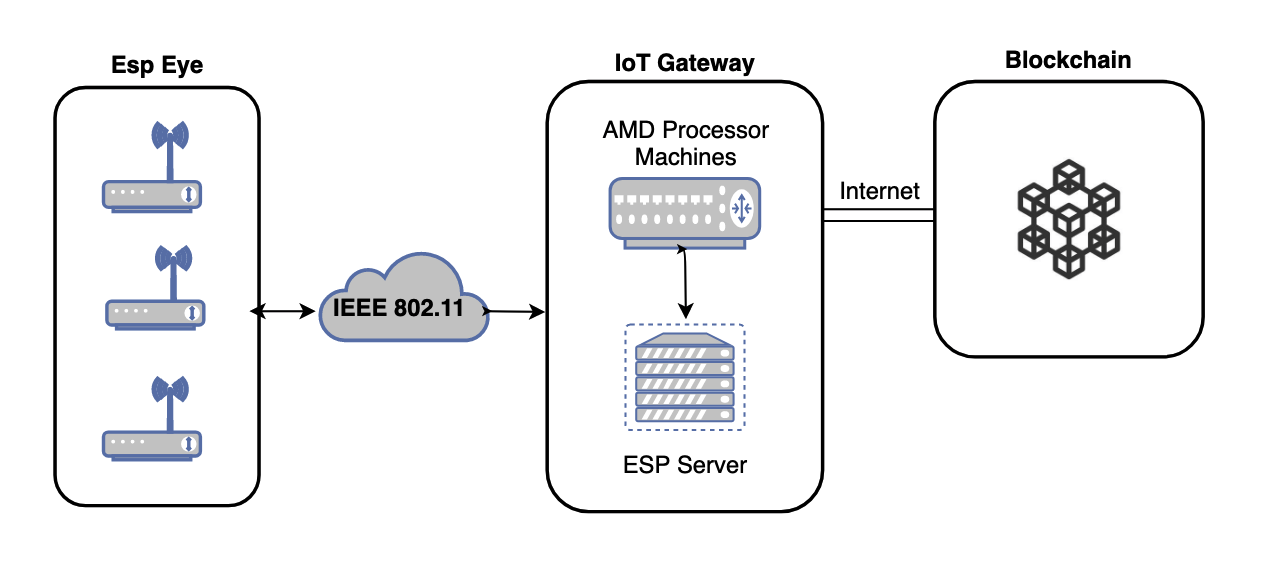
\includegraphics[width=1\textwidth]{figures/dataflow.png}
    \caption{Data flow diagram}
    \label{fig:dataflow}
\end{figure}
The nodejs server is responsible for receiving the data and forwarding it to the Hyperledger Fabric. 
In order to interact with Fabric blockchain network the Fabric SDK for nodejs provides us with APIs to submit transactions to the ledger. The process of submission takes place right after the image has arrived. Hyperledger ledger data is known as assets which are represented as as a collection of key-value pairs. When the value of the key is modified by a chaincode simulated from transaction execution then the world state is updated as a new transaction on a ledger. Assets written by chaincode typically use the JSON form and or binary. Since for the backend the JSON format is used for file transfer then this allows for sending the same JSON parameters to the blockchain. The role of nodejs server is to receive and acknowledge the Esp Eye that data has arrived and then forward the exact same data to the blockchain. The process begins with transaction initiation where Esp Eye is assumed to be a client and such that it holds an identity issued from the MSP. 

A question may arise why are we storing the image directly in the blockchain. First Hyperledger Fabric runs at no costs for transaction execution and the consensus mechanism is very lightweight and pluggable. Secondly, since Hyperledger Fabric allows for splitting the network into multiple smaller networks in order to preserve privacy between competitors then storing images in some other third party such as IPFS would vaporize the concept of channeling and IPFS does not offer the same characteristics. 


\subsection{Transmission Overview}
\subsubsection{Esp Eye starts video surveillance}
The data transmission is depicted in Figure~\ref{fig:seqdiag} which captures the interaction between all the components end to end. When an Esp Eye device established connection to the LAN it then immediately start the process of video surveillance. Roughly it takes 4 frames per second and analysis each frame for face detection and if a face is detected only then it puts into work the face recognition algorithm. Only if a face is detected or eventually recognized the client code will be activated and eventually through an end point using the POST method. 






\begin{figure}[!htb]
    \centering
    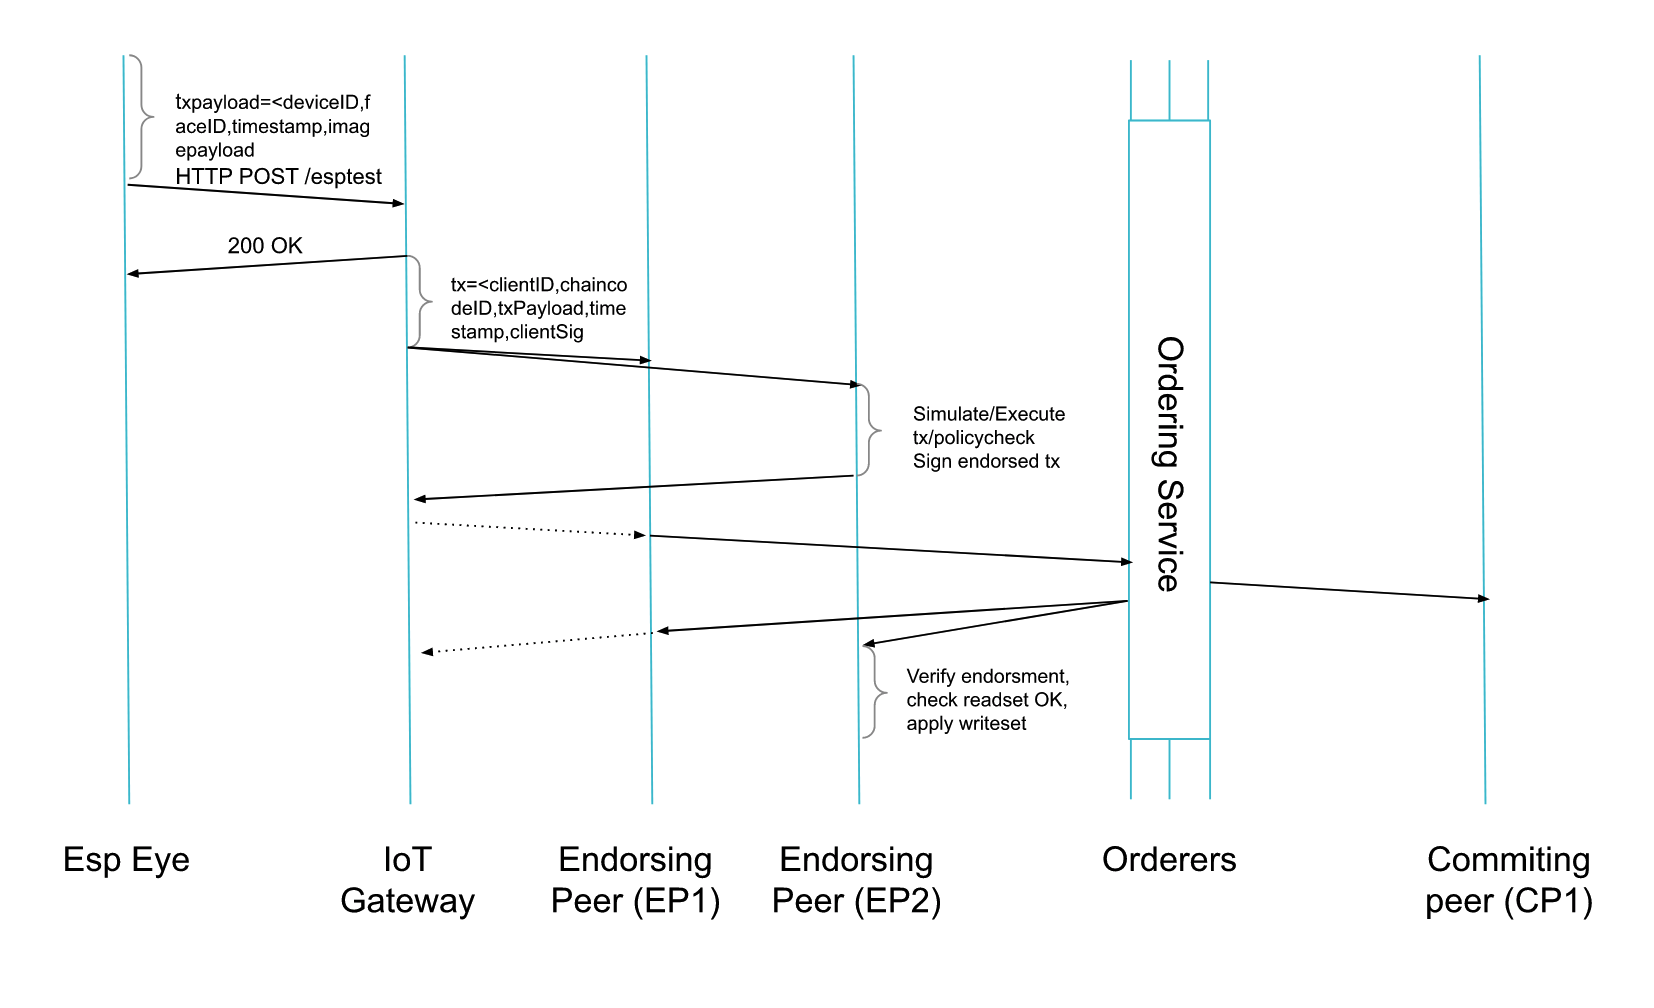
\includegraphics[width=1\textwidth]{figures/sequencediagram1.png}
    \caption{Sequence Diagram showing transaction execution}
    \label{fig:seqdiag}
\end{figure}




There are 4 important information needed to be stored in the blockchain and are reflected in the Figure~\ref{fig:json}. First the DeviceID is important since we need to know from which device is this information coming as multiple devives may be employed in video surveillance. Secondly with FaceID we will be able to identify the person without having to look on the captured frame. Additionaly with timestamp we capture the time when the person is detected and finally the frame itself encoded in base64. 

As in Figure~\ref{fig:seqdiag} these 4 parameters will be sent first through the exposed API with an endpoint /esptest. The nodejs server located in IoT Gateway will then reply with the status code but no additional information. 

\begin{figure}[!htb]
    \centering
    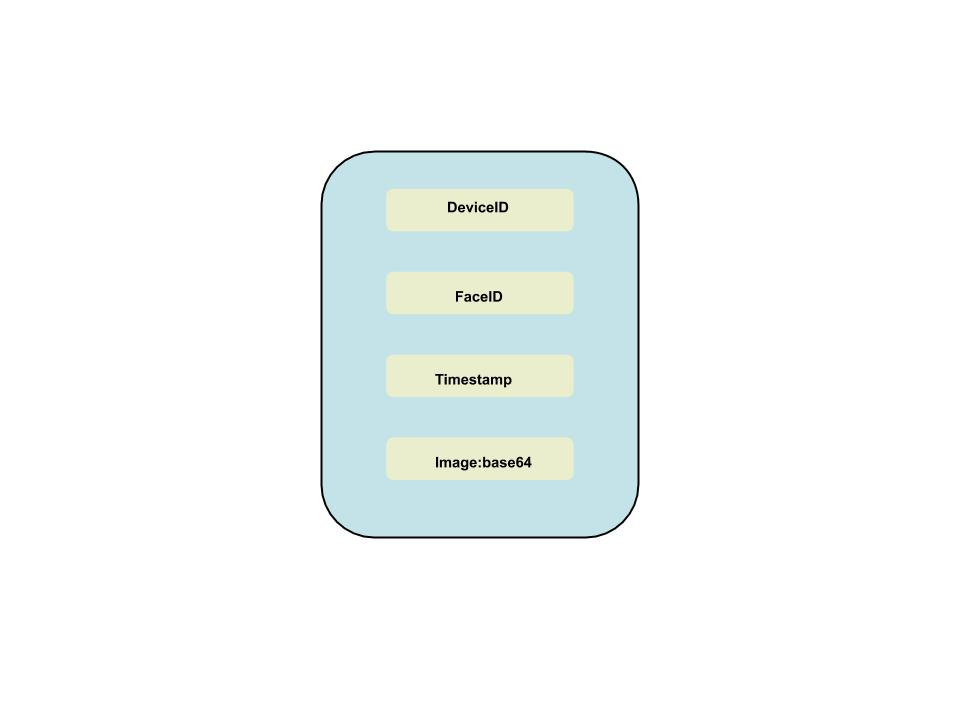
\includegraphics[width=1\textwidth]{figures/json2.jpg}
    \caption{JSON parameters sent from Esp Eye}
    \label{fig:json}
\end{figure}
\subsubsection{IoT Gateway initiates a transaction}
Before transaction is initiated there are three assumptions necessary to keep in mind:
\begin{itemize}
    \item The channel in Fabric is running.
    \item The Esp Eye is registered and enrolled with Certificate Authority and MSP holds its identity.
    \item The chaincode with its endorsement policy is deployed on the peers.
\end{itemize}


Now the job of the IoT Gateway is to initiate the transaction with the 4 paremeters passing them as they are to the transaction payload. The IoT Gateways acts as a Fabric client for Hyperledger Fabric. Our endorsement policy states that both peers taking part in the consortium must endorse any transaction coming from this client. The transaction proposal now is easy constructed, since Fabric holds assets in key value pairs in our case the key will be the FaceID and all other information will be stored in a json document as values. This will make it easier to query the FaceIDs and for the world state. The transaction proposal utilizes an API for nodejs SDK to generate a transaction. The goal of the API which we are going to see its implementation soon is to invoke the functions of the chaincode with input paramters coming from Esp Eye. Each Esp Eye is issued a public private key pair which is used to sign the transaction before sending it to the endorsers for execution. In this case the Fabric-client SDK persists the public private key and signs the transaction on behalf of the Esp Eye. Although transaction signing is possible in offline mode which means the user signs the transaction at his device and sends the signed transaction to the endorser node. In our case this was not possible since the Fabric-client SDK is not available for Esp Eye devices. 

\subsubsection{Endorsing Peers EP1 and EP2 verify and execute the transaction}

The endorser EP1 and EP2 from Figure~\ref{fig:seqdiag} will now receive the transaction proposal which includes: clientID, chaincodeID, txPayload, timestamp and clientSignature as in Figure~\ref{fig:endorsejson}. Only the endorsing peers specified by the chaincode will receive this transaction proposal in our case both of them will receive a proposal. EP1 and EP2 first of all check the format of the transaction and if the signature is valid and if that is the client who claims to be using the MSP. Besides it also ensures that this client in this case Esp Eye is an authorized member of that channel. When all the conditions have passed then the endorses invokes the chaincode function and pass the four proposed arguments. Eventually the transaction is executed however it does not yet update the ledger. Now the endorsers sign the proposed transaction and send back a proposal response to the fabric-client. The intent of the fabric-client now is to submit the transaction to the ordering service to update the ledger. If the fabric-client was to query the ledger then there is no need to submit anything to the ordering service. However in order for the fabric-client to submit the transaction to the ordering service both endorser EP1 and EP2 have to respond with same response proposal. However yet at this stage the ledger is not updated. 

\begin{figure}[!htb]
    \centering
    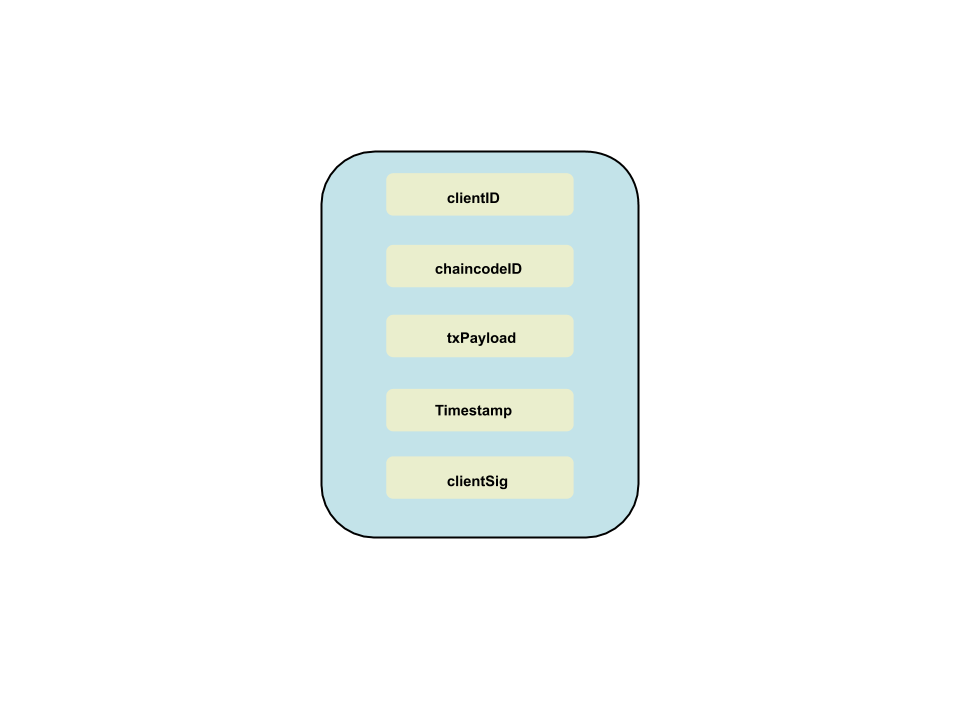
\includegraphics[width=1\textwidth]{figures/endorsejson.png}
    \caption{Proposed transaction with its parameters.}
    \label{fig:endorsejson}
\end{figure}


\subsubsection{Fabric-client submits transactions to the ordering service}

Before the fabric-client submits the final version of the transaction, the application broadcasts the endorsed transaction with a message to the ordering service.
The transaction proposal now will contain the read/write sets besides the endorsing peers signatures. 
The ordering service nodes may receive transaction from other clients or other ESP devices. The job of the ordering service is to order transactions on an agreed sequence in order to package them into blocks. After the maximum number of transactions allowed in a blocks is reached or the maximum time duration has passed then blocks are saved first to the ledger of the orderers. 


\subsubsection{Validate and commit the transactions to all peers}

Upon receiving a broadcast message with the created block from the orderers the committing peers will again verify the signatures of the ordering nodes which are part of the ordering service. In Fabric it is allowed to set which peers will validate the transaction and they are name as committing peers, however all the peers in the channel ought to update the ledger.
If the committing peers fail to verify the signature of the ordering peers that created the block then the block is rejected for inclusion in the ledger. Another very important validation step is to ensure that every transactions' read and write set does not lead to invalid world state. During the endorsement phase the every transaction copies a set of read and write sets of the key pair that will get updated. Hyperledger Fabric in addition to key value pairs it implicitly keeps the third parameter which is the version number of that pair. When a new transaction is executed the versioning  of the key pair gets updated, it is like a counter. The read set comes from the world state and the write set is the same key but with updated value and version. In our case the key will be the FaceID and the value is the new image.

The committing/validating peers will now verify the transaction by looking at the read write sets. Now the committing peer will compare the read set it holds with the world state of the same key. If the versioning of the key does not match then a previous transaction could have updated and the version is also updated which means the transaction will be considered invalid and will be rejected from the block. This is how it prevents the double spending. Otherwise if the read set and its version has not been changed the transaction is then allowed to be inserted to the ledger. Eventually the write sets are committed to the world state and the detected image has reached all the peers. 
 
 \subsubsection{Execution model}
 
 
 Typically the permissioned blockchains such as Ethereum, the transaction is executed by all peers in the block level which means that the consensus protocol first orders the transactions and propagates to the peer nodes and only then the execution of transactions takes place. Therefore they operate in order-execute-validate model. The execution happens after all the transactions have been propagated to all peers by executing sequentially all the transactions in all peers.
 
 Unlike the traditional approaches, Hyperledger Fabric follows the execute-order-validate model which is reflected in the above described steps. This model has a lot of advantages. First of a transaction is not executed by all the peers but only by a subset of the peers. Besides also the transaction endorsement and validation may be executed only by a subset of the peers which means not all the peers need to execute the chaincode. Since many peers are released from the transaction execution this can save energy and resources because some of the peers may be running far away from each other. 
 This approach uses a non-deterministic chaincode because the peer agreement is explicit  which allows to implement the chaincode in a non-deterministic programming language. In addition the Fabric allows to execute transactions in parallel in order to increase throughput. Besides the elapsed timeout for a block creation makes Hyperledger Fabric much more efficient for transactions coming from IoT devices.
 
 
 
\subsection{Esp Eye Setup}

In the previous section with a sequence diagram the data flow from one object to another is elaborated. In this section we would like to stop on the most important parts of the implementation for face detection and recognition which is entirely implemented using Arduino IDE. Since three domains are involved we wouldn't be able to elaborate all the details here because the focus is merely on the interactions between them. Because of that the face detection and recognition algorithms implemented in Esp Eye are shown in more detail in Chapter 3. Therefore we will now take a look at the most important parts of implementation which runs face detection and recognition.

%First of all the implementation begins with setting the GPIO parameters in order to connect to camera. This is important because each ESP32 camera board uses different GPIOs. Now we would like to fave a close look at the APIs used for face detection and recognition.

\subsubsection{Face Detection API} 

First of all we would like to start with introduction to the API for face detection: {\fontfamily{ccr}\selectfont face\_detect} which is adapted from ESP WHO platform, its implementation is shown in the Listing \ref{face_detect}. As it can be seen the function returns a pointer of type {\fontfamily{ccr}\selectfont box\_array\_t} which contains information about the face such as the bounding box and the face landmarks. When no face is detected the function returns {\fontfamily{ccr}\selectfont NULL}. In our code we just check if the the function returns {\fontfamily{ccr}\selectfont NULL} then do not proceed for face recognition. The {\fontfamily{ccr}\selectfont face\_detect} function accepts to inputs of type {\fontfamily{ccr}\selectfont dl\_matrix3du\_t} and {\fontfamily{ccr}\selectfont mtmn\_config\_t}. 


\begin{lstlisting}[caption={Face detection API},label=face_detect, captionpos=b]

// Adapted from ESP-WHO Platform
 box_array_t *face_detect(dl_matrix3du_t *image_matrix, mtmn_config_t *config)
{ 
    net_config_t pnet_config = {0};
    pnet_config.w = 12;
    pnet_config.h = 12;
    pnet_config.threshold = config->p_threshold;
    box_array_t *pnet_boxes = NULL;
    if (FAST == config->type)
        pnet_boxes = pnet_forward_fast(image_matrix,
                                       config->min_face,
                                       config->pyramid_times,
                                       &pnet_config);
    else if (NORMAL == config->type)
        pnet_boxes = pnet_forward2(image_matrix,
                                   config->min_face,
                                   config->pyramid,
                                   config->pyramid_times,
                                   &pnet_config);
    if (NULL == pnet_boxes)
        return NULL;
    net_config_t rnet_config = {0};
    rnet_config.w = 24;
    rnet_config.h = 24;
    rnet_config.threshold = config->r_threshold;
    box_array_t *rnet_boxes = rnet_forward(image_matrix,
                                           pnet_boxes,
                                           &rnet_config);
    dl_lib_free(pnet_boxes->box);
    dl_lib_free(pnet_boxes);

    if (NULL == rnet_boxes)
        return NULL;
    net_config_t onet_config = {0};
    onet_config.w = 48;
    onet_config.h = 48;
    onet_config.threshold = config->o_threshold;

    box_array_t *onet_boxes = onet_forward(image_matrix,
                                           rnet_boxes,
                                           &onet_config);
    dl_lib_free(rnet_boxes->box);
    dl_lib_free(rnet_boxes);
    return onet_boxes;
} /*}}}*/
\end{lstlisting}






The Listing \ref{image_matrix} shows the definition of the image\_matrix a 3 dimensional matrix with the image and additional metadata about the image unlike the {\fontfamily{ccr}\selectfont box\_array\_t} which only holds features about the face. These are information about the image width, height, number of channels, number of filters, stride and a pointer to image data. Since we are dealing with a memory constraint device typically the dynamic memory allocation is used. It allows for more efficient memory allocation and the memory is not wasted. So first the memory is dynamically allocated and then the captured image is assigned to it. 




\begin{lstlisting}[caption={Image matrix structure},label=image_matrix, captionpos=b]
typedef struct
{
    int w;      /*!< Width */
    int h;      /*!< Height */
    int c;      /*!< Channel */
    int n;      /*!< Number of filter, input and output must be 1 */
    int stride; /*!< Step between lines */
    uc_t *item; /*!< Data */
} dl_matrix3du_t;

\end{lstlisting}


The second parameter {\fontfamily{ccr}\selectfont mtmn\_config\_t} also shown in Listing \ref{mtmn} is a struct which holds configurations about the MTMN, the multi stage algorithm for face detection which is explained in detail in Chapter 3. There are a number of properties which are important because they can affect the performance of MTMN and also the processing speed. The first property is 
{\fontfamily{ccr}\selectfont min\_face} which is the minimum detection size which by default is set to 80. It means that it should be able to detect all faces larger than 80x80 pixels. This property is important since we do want to detect individual faces and anyone standing in the background is not important. Therefore the smaller the {\fontfamily{ccr}\selectfont min\_face} is : 

\begin{itemize}
    \item the larger the number of images is generated in image pyramid;
    \item the higher the processing time;
     \item the smaller the size of detectable face is in the image;
\end{itemize}


In other words it means the MTMN will work harder to try to detect the face if the person is standing pretty far away from the camera. 
The {\fontfamily{ccr}\selectfont pyramid} holds the scale which monitors the generated pyramids with a range from 0 to 1. 

Therefore the larger the {\fontfamily{ccr}\selectfont pyramid} is : 
\begin{itemize}
    \item the higher the number of images generated in the image pyramid;
    \item the higher the processing time;
\end{itemize}

The {\fontfamily{ccr}\selectfont pyramid\_times} is another property which together with {\fontfamily{ccr}\selectfont pyramid} monitor the image pyramid. In addition the configuration also allows to set the threshold for each stage of the MTMN reflected in the struct {\fontfamily{ccr}\selectfont threshold\_config\_t}. The closer to 1 the lower the number of potential candidate bounding boxes and such the lower the probability of detecting a face. 
The struct {\fontfamily{ccr}\selectfont mtmn\_resize\_type} allows to chose between FAST and NORMAL. When it is set to FAST the {\fontfamily{ccr}\selectfont pyramid} equals 0.707106781. If we want to set out own value of {\fontfamily{ccr}\selectfont pyramid} the it has to be set to NORMAL. By FAST it means the processing time is faster compare to NORMAL. 


\begin{lstlisting}[caption={MTMN configurations },label=mtmn, captionpos=b]
 typedef struct
    {
        float min_face;                 /*!< The minimum size of a detectable face */
        float pyramid;                  /*!< The scale of the gradient scaling for the input images */
        int pyramid_times;              /*!< The pyramid resizing times */
        threshold_config_t p_threshold; /*!< The thresholds for P-Net. For details, see the definition of threshold_config_t */
        threshold_config_t r_threshold; /*!< The thresholds for R-Net. For details, see the definition of threshold_config_t */
        threshold_config_t o_threshold; /*!< The thresholds for O-Net. For details, see the definition of threshold_config_t */
        mtmn_resize_type type;          /*!< The image resize type. 'pyramid' will lose efficacy, when 'type'==FAST. */
    } mtmn_config_t;
    
\end{lstlisting}
%and then we will see each arguments are expected for face detection. 

In the Listing \ref{face_detect}  of the {\fontfamily{ccr}\selectfont face\_detect} function the three stages of MTMN are implemented. As discussed in Chapter 3 in the p-net stage the input image size is 12x12 this is reflected with assigning the {\fontfamily{ccr}\selectfont pnet\_config.w} and {\fontfamily{ccr}\selectfont pnet\_config.h} to 12. Similarly this happens for r-net and o-net where the width and height is set to 24x24 and 48x48 respectively. Once the function has reached the end it will return either NULL if no face is detected or else will return the bounding box, the score and landmarks.


\subsubsection{Face Recognition API} 

The input for face recognition is only the bounding box or the aligned face with landmarks for the position of eye,nose and mouth. The {\fontfamily{ccr}\selectfont recognize\_face} function accepts two parameters, the {\fontfamily{ccr}\selectfont face\_id\_list} and the {\fontfamily{ccr}\selectfont aligned\_face}.
\begin{lstlisting}[caption={Face Recognition API},label=face_rec, captionpos=b]
int8_t recognize_face(face_id_list *l, dl_matrix3du_t *algined_face);
\end{lstlisting}

The face id list also shown in Listing \ref{face_id} has a number of parameters that keeps track of the face ids, where the most important information about the face is stored in a 3 dimensional vector {\fontfamily{ccr}\selectfont id\_list}. 





\begin{lstlisting}[caption={Face Id List},label=face_id, captionpos=b]
typedef struct
  {
        uint8_t head;            /*!< head index of the id list */
        uint8_t tail;            /*!< tail index of the id list */
        uint8_t count;           /*!< number of enrolled ids */
        uint8_t size;            /*!< max len of id list */
        uint8_t confirm_times;   /*!< images needed for one enrolling */
        dl_matrix3d_t **id_list; /*!< stores face id vectors */
    } face_id_list;
    
    \end{lstlisting}

The job of {\fontfamily{ccr}\selectfont recognize\_face} function is to generate a new {\fontfamily{ccr}\selectfont face\_id} from the {\fontfamily{ccr}\selectfont aligned\_face} parameter. The newly generated {\fontfamily{ccr}\selectfont face\_id} will then be compared with all the face ids stored in the {\fontfamily{ccr}\selectfont face\_id\_list}. With the help of Cosine similarity we can measure how similar two vectors are. The Cosine similarity will then obtain the distance between the newly generated {\fontfamily{ccr}\selectfont face\_id} with each {\fontfamily{ccr}\selectfont face\_id} stored in the {\fontfamily{ccr}\selectfont face\_id\_list}. The closer the Cosine value to 1 the higher the match between two vectors and vice versa. As a matter of fact it is almost impossible to have a Cosine value 1 of two compared faceIDs. This is challenging due to image differences in terms of light, pose and facial expression. Due to that we can set a threshold {\fontfamily{ccr}\selectfont FACE\_REC\_THRESHOLD}  to either increase or decrease the recognition rate. When it obtains a Cosine value greater than the threshold when comparing two face IDs then it is considered to be the same person. 

\subsubsection{Sending detected image to IoT Gateway} 

The image is sent to IoT Gateway either when a face is detected or recognized. The WiFiClient library in Arduino enables to establish the connection to the IoT Gateway by using the IP address of the IoT Gateway. The Esp Eye makes an HTTP request using the POST method through an exposed API from the IoT Gateway. Throughout this study for submitting the image to the IoT Gateway two ways were used: 
\begin{enumerate}
    \item multipart/form-data
    \item application/json
\end{enumerate}

With "multipart/form-data" the image is sent in series of parts. This approach allows to send a file or image without looking at its type. This approach was used at the beginning of the project implementation when a python server was used and such that we did not have information about the Hyperledger Fabric implementation which uses Javascript for interaction with blockchain. This approach is beneficial when we do not want to capture the raw image in bytes. 

The second approach "application/json" is a standard format of sending structured data. It is useful for sending plain text or any other type of data. Since Hyperledger Fabric also uses JSON format to store assets and the only way to store the image in it is to convert the image in data type JSON supports. Hence the best option is to store it as a String and to do that the image is first converted to {\fontfamily{ccr}\selectfont base64} and when needed we can convert it back to an image type. So then we decided to do the conversion in Esp Eye itself and send the image as {\fontfamily{ccr}\selectfont base64} using JSON format. 
The Listing \ref{json_esp} shows the parameters that are being sent to the IoT Gateway and the exact same parameters are inserted into Fabric ledger.
\begin{lstlisting}[caption={JSON structure in Esp Eye},label=json_esp, captionpos=b]
{
        DeviceId: 
        Face_Id: 
        Timestamp: 
        ImageData: 
}

\end{lstlisting}


\subsection{IoT Gateway}

The IoT Gateway holds two important components, the nodejs server and the Hyperledger Fabric SDK that serves as the client for Hyperledger Fabric blockchain. The Express.js an application server framework enables to build the server in nodejs. With an exposed API in nodejs the Esp Eye will be able to send the data as in the Listing\ref{api_test}. The nodejs server will then pass the data to the Hyperledger Fabric SK for further propagation to the ledger.



\begin{lstlisting}[caption={The exposed API for handling requests coming from Esp Eye},label=api_test, captionpos=b]
app.post("/esptest", async (req, res) => {

    if (req.body.ImageData) {
        console.log(" Device Id is:-", req.body.DeviceId);
        console.log(" Face id is :-", req.body.Face_Id);
        console.log(" Base64 Image is:-", req.body.ImageData);
        console.log(" Date Time is:-", req.body.Timestamp);
    }

    res.sendStatus(200);
    console.log("Receided image and uploading to blockchain");
    main(req.body.Face_Id, req.body.DeviceId, req.body.Timestamp, req.body.ImageData);
});
\end{lstlisting}



\subsection{Hyperledger Fabric Setup}
Hyperledger Fabric allows two or multiple organisations to be part of the ledger and the transaction lifecycle. In our use case of video surveillance we have two organisations and each organisation has one peer. The first organisation can be the institute itself which is willing to use and deploy the video surveillance and the other organisation would be the surveillance company which is monitoring the access control. 

The Hyperledger Fabric implementation has two parts of the code: the Chaincode implementation and the client implementation. 

\subsubsection{Chaincode implementation}

The Chaincode implementation which is deployed and executed inside the network is shown in the Listing \ref{chaincode}. First of all the {\fontfamily{ccr}\selectfont fabric-contract-api} module for nodejs is used for the implementation of Hyperledger Fabric chaincode which provides the {\fontfamily{ccr}\selectfont Contract} interface. This API provides an entry to write the chaincode functions in order to allow the endorsing peers and blockchain clients to communicate. Hyperledger Fabric makes it possible to write chaincode in Go, Java and Javascript (nodejs). One of the biggest advantage is that no matter in which of the above languages the chaincode is implemented, it still allows the client to use a different language for communication but it has to be among one of the mentioned programming language. 
Hence we decided to go for Javascript implementaion of the chaincode since the client is also implemented in Javascript. 

There are a number of functions implemented each with its own purpose which can be split into two categories, the functions for inserting images into the ledger and querying images from the ledger.  For inserting images coming from the Esp Eye the {\fontfamily{ccr}\selectfont create\_Image} function is implemented. This function receives five arguments: {\fontfamily{ccr}\selectfont ctx}, {\fontfamily{ccr}\selectfont faceid}, {\fontfamily{ccr}\selectfont device\_id}, {\fontfamily{ccr}\selectfont timestamp} and the {\fontfamily{ccr}\selectfont imageitself}.
The first argument {\fontfamily{ccr}\selectfont ctx} is the transaction context which keeps the state of the transaction. First of all it allows to maintain variables when invoking transactions. Secondly it offers a number of very important APIs to establish communication and perform transaction processing. As you can see in the Listing \ref{chaincode} {\fontfamily{ccr}\selectfont ctx.stub.putState} function assembles the arguments into key value pairs, where the key is the {\fontfamily{ccr}\selectfont faceid} and the rest of arguments will be inserted as values to that key. The {\fontfamily{ccr}\selectfont ctx.stub} is used to access the 
{\fontfamily{ccr}\selectfont putState} API which writes to the ledger. Besides {\fontfamily{ccr}\selectfont ctx.stub} provides very important APIs for inserting into the ledger and querying it.  










\begin{lstlisting}[caption={Chaincode for interacting with the network.},label=chaincode, captionpos=b]

'use strict';
const { Contract } = require('fabric-contract-api');

class FabImages extends Contract {

    async initLedger(ctx) {
        console.info('============= START : Initialize Ledger ===========');
        const images = [
            {
                device_id: 'Device 1',
                timestamp: '2020 - 12 - 13T01: 47: 38Z',
                docType: 'image',
                imageitself: 'AAAFCAYAAACNbybl',

            }
        ];

        for (let i = 0; i < images.length; i++) {
            images[i].docType = 'image';
            await ctx.stub.putState('Face id 0', Buffer.from(JSON.stringify(images[i])));
            console.info('Added <--> ', images[i]);
        }
        console.info('============= END : Initializing Ledger ===========');
    }

    async queryImage(ctx, faceid) {
        const imageAsBytes = await ctx.stub.getState(faceid); // get the image from chaincode state
        if (!imageAsBytes || imageAsBytes.length === 0) {
            throw new Error(`${faceid} does not exist`);
        }
        console.log(imageAsBytes.toString());
        return imageAsBytes.toString();
    }

    async createImage(ctx, faceid, device_id, timestamp, imageitself) {
        console.info('============= START : Create Image ===========');

        const image = {
            device_id,
            timestamp,
            docType: 'image',
            imageitself

        };

        await ctx.stub.putState(faceid, Buffer.from(JSON.stringify(image)));
        console.info('============= END : Create Image ===========');
    }

    async queryAllImages(ctx) {
        const startKey = '';
        const endKey = '';
        const allResults = [];
        for await (const { key, value } of ctx.stub.getStateByRange(startKey, endKey)) {
            const strValue = Buffer.from(value).toString('utf8');
            let record;
            try {
                record = JSON.parse(strValue);
            } catch (err) {
                console.log(err);
                record = strValue;
            }
            allResults.push({ Key: key, Record: record });
        }
        console.info(allResults);
        return JSON.stringify(allResults);
    }

    async retrieveHistory(ctx, key) {
        console.info('getting history for key: ' + key);
        let iterator = await ctx.stub.getHistoryForKey(key);
        let result = [];
        let res = await iterator.next();
        while (!res.done) {
            if (res.value) {
                console.info(`found state update with value: ${res.value.value.toString('utf8')}`);
                const obj = JSON.parse(res.value.value.toString('utf8'));
                result.push(obj);
            }
            res = await iterator.next();
        }
        await iterator.close();
        return result;
    }

    async query(ctx, key) {
        console.info('querying for key: ' + key);
        let returnAsBytes = await ctx.stub.getState(key);
        let result = JSON.parse(returnAsBytes);
        return JSON.stringify(result);
    }

    async querySpecificKey(ctx, key) {
        console.info('querying for key: ' + key);
        let returnAsBytes = await ctx.stub.getState(key);
        let result = JSON.parse(returnAsBytes);
        return result;
    }
}

module.exports = FabImages;

\end{lstlisting}


Other functions implemented in the chaincode are useful for querying the ledger in different ways. For instance the function {\fontfamily{ccr}\selectfont queryAllImages}  retrieves the world state of all key pairs in the ledger. This is has been useful for testing purposes. In this case the function {\fontfamily{ccr}\selectfont getStateByRange} API is used to iterate over all sets of keys from the startKey until the endKey. 
Additionally the functions {\fontfamily{ccr}\selectfont querySpecificKey} allows to query the world state of a specific key. This is achieved with the help of {\fontfamily{ccr}\selectfont ctx.stub.getState} API which retrieves the current value of the passed key. When we want to see the history of all values for a key the function function {\fontfamily{ccr}\selectfont retrieveHistory} can be used which takes in a key and returns the entire history of all values ever inserted for given key. 

\subsubsection{Hyperledger Fabric Client implementation}
The Hyperledger Fabric Client is how the outside world interacts with the blockchain network. In order for the client to interact with the Fabric network and chaincodes the {\fontfamily{ccr}\selectfont fabric-network} module for nodejs is used. Typically in Bazo blockchain and Ethereum a developer need to know the exposed gateway to interact with the network which normally the RESTfull services are used. 

Hyperledger Fabric offers a number of classes through the module {\fontfamily{ccr}\selectfont fabric-network} for nodejs to make calls to the network. The most important class of this module is {\fontfamily{ccr}\selectfont Gateway}. It includes various methods to establish connection and interaction with the fabric network. The Listing \ref{client_connect} shows snippets of the client implementation. First of all the existing participant in our case the Esp Eye is a participant. This participant is connected to the fabric network in the right channel and will be allowed to access a particular chaincode which are all defined previously in the participant's access rights. Once the connection is established then the participant or client is allowed to submit transactions. Then the {\fontfamily{ccr}\selectfont submitTransaction} function will submit a transaction to the peeers (endorser) using a specified function of a chaincode by passing arguments needed for the function being used.  The transaction function will then be evaluated by the endorsing peers which will then further be submitted to the ordering service to eventually be inserted into ledger. 


\begin{lstlisting}[caption={Client establishing the connection and submitting a transaction.},label=client_connect, captionpos=b]
        // Create a new gateway 
        const gateway = new Gateway();
        await gateway.connect(ccp, { wallet, identity: 'appUser', discovery: { enabled: true, asLocalhost: true } });

        // Get the network (channel) where the contract is deployed.
        const network = await gateway.getNetwork('mychannel');

        // Get the contract.
        const contract = network.getContract('imagecontractupdated');

        // Submit a transaction.
        await contract.submitTransaction('createImage', faceid, deviceid, timestamp, imagebase64);
        console.log('Transaction has been submitted');

        // Disconnect from the gateway.
        await gateway.disconnect();
\end{lstlisting}

We have seen now how a transaction is submitted using the {\fontfamily{ccr}\selectfont fabric-network} module. In order to retrieve and check that what have been submitted is in the ledger we can take the advantage of {\fontfamily{ccr}\selectfont evaluateTransaction} method. The purpose of this method is to query the ledger using the functions in the chaincode which resembles the GET method in HTTP requests. The chaincode function will only be evaluated by the endorsing peers and will not involve the ordering service and there will be no changes to the ledger state. 

\subsection{Frontend Implementation}

Considering that the image from its origin Esp Eye until it reaches the blockchain is of type {\fontfamily{ccr}\selectfont base64} and we are not able to see visually anything for that reason a web application is developed. For the development of web application we are using react Javascript library. The web application will take the advantage of the same local nodejs server for the backend. In the nodejs server we have exposed another gateway which can be seen in the Listing \ref{frontend}. 
The client can retrieve the image in base64 from the ledger by making a single REST call using the GET method. The {\fontfamily{ccr}\selectfont getFile} endpoint will expect a key which is the faceID of a person. After that another client for Hyperledger Fabric is employed which actually is the same client (participant) which inserts images to the ledger. Similarly as in the Listing \ref{client_connect} the client first establishes the connection and only then can query the ledger. As already mentioned the {\fontfamily{ccr}\selectfont evaluateTransaction} method of the {\fontfamily{ccr}\selectfont contract} instance allows to read the ledger state.  

\begin{lstlisting}[caption={The API gateway serving the web application.},label=frontend, captionpos=b]

app.get("/getFile", async (req, res) => {
    if (req.query.filehash) {
        const chunks = [];
        console.log("Key value:", req.query.filehash);
        //let key = 'Face_id_0';
        const result = await queryfrontend.main(req.query.filehash);
        console.log(result);
        res.send(result);
        // res.send(Buffer.concat(chunks).toString());
    } else {
        res.status(501).send("Please provide face id");
    }
});

\end{lstlisting}

To retrieve the image the client has to query the ledger which means that we need to have a method in the chaincode to do so. Since we have implemented one chaincode then the method is reflected in the Listing \ref{chaincode} with the name {\fontfamily{ccr}\selectfont querySpecificKey}. The function expect the faceID of the person and only then the image will be returned to the client and be displayed on the web client. 









